%\chapter{Ứng dụng đạo hàm để khảo sát và vẽ đồ thị của hàm số}
%\section{Tính đơn điệu và cực trị của hàm số}
%\subsection{Tóm tắt lý thuyết}
%\begin{tomtat}
%	\subsubsection{Tính đơn điệu của hàm số}
%	
%	\subsubsection{Cực trị của hàm số}
%\end{tomtat}

%\chude{Xét tính đơn điệu và cực trị của hàm số}

%\begin{tomtat}
%	Để xét tính đồng biến, nghịch biến và điểm cực trị của hàm số $y=f\left(x\right)$, ta có thể thực hiện các bước sau
%\end{tomtat}
%\begin{dang}{Xét tính đơn điệu và cực trị của hàm số khi biết bảng biến thiên hoặc đồ thị hàm số $y=f\left( {x} \right)$}
%\end{dang}
%\vande{Tên vấn đề (nếu có)}

\TNSA

\Opensolutionfile{ans}[ans/ans-2-B1]

\begin{ex}%[2H5C3-3]
	Trong không gian với hệ trục toạ độ $Oxyz$ cho mặt phẳng $(Q)$ có phương trình $x-2y+z-5=0$ và mặt cầu $S$ có phương trình $(x-1)^2 + y^2 + (z + 2)^2 = 15$. Mặt phẳng $\left(P\right)$ song song với mặt phẳng $\left(Q\right)$ và cắt mặt cầu $(S)$ theo giao tuyến là một đường tròn có chu vi bằng $6\pi$. Gọi phương trình của mặt phẳng $\left(Q\right)$ có dạng $x + by + cz + d = 0$, tính giá trị $V = a + b + c + d$.
	
	\shortans{$7$}
	
	\loigiai{Mặt cầu $\left(S\right)$ có tâm $I(1;0;-2)$ và bán kính $R = \sqrt{15}$. \\
	Đường tròn có chu vi bằng $6\pi$ nên có bán kính là $r = \dfrac{6\pi}{2\pi} = 3$. \\
	Mặt phẳng $\left(P\right)$ song song với mặt phẳng $\left(Q\right)$ nên phương trình mặt phẳng $\left(P\right)$ có dạng: $x - 2y + z +d = 0$ ($d \ne -5$).
	\begin{equation*}
		\begin{split}
			\mathrm{d}\left(I; \left(P\right)\right) = \sqrt{R^2 - r^2} &\Leftrightarrow \mathrm{d}\left(I; \left(P\right)\right) = \sqrt{6}
			\\ &\Leftrightarrow \frac{\left| {1 - 2.0 - 2 + d} \right|}{\sqrt {1^2 + \left(-2 \right)^2 + 1^2}} = \sqrt 6
			\\ &\Leftrightarrow \left| {d - 1} \right| = 6
			\\ &\Leftrightarrow \hoac{
				&d - 1 = 6 \\
				&d - 1 =  - 6. \\ }
			\\ &\Leftrightarrow \hoac{
				&d = 7 \\
				&d =  - 5. \\ 
		}
		\end{split}
	\end{equation*}
	
	\noindent Đối chiếu điều kiện, ta tìm được $d=7$. Vậy $\left(P\right)$ có phương trình là $x-2y+z+7=0$. Suy ra $V = 1 - 2 + 1 + 7 = 7$. 
	}
\end{ex}

\begin{ex}%[2H5C3-3]
	Trong không gian với hệ trục toạ độ $Oxyz$ cho mặt cầu $\left(S\right)$ có phương trình $(x-1)^2 + (y - 2)^2 + (z-3)^2 = 1$ và điểm $A(2;3;4)$. Biết tập hợp điểm $M$ thuộc $\left(S\right)$ sao cho đường thẳng $AM$ tiếp xúc với $\left(S\right)$ là mặt phẳng có phương trình $x + by + cz + d = 0$. Tính giá trị $V = a \cdot b \cdot c \cdot d$.
	
	\shortans{$-7$}
	
	\loigiai{Mặt cầu $\left(S\right)$ có tâm là $I(1;2;3)$ và bán kính là $1$. Dễ thấy điểm $A$ nằm ngoài mặt cầu $\left(S\right)$. \\
	Đường thẳng $AM$ tiếp xúc với $\left(S\right)$ khi và chỉ khi $AM \perp IM \Leftrightarrow \overrightarrow{AM} \cdot \overrightarrow{IM} = 0$.
	\begin{equation*}
		\begin{split}
			&\Leftrightarrow \left(x - 2\right)\left(x - 1 \right) + \left(y - 3 \right)\left( y - 2 \right) + \left(z - 4 \right)\left(z - 3 \right) = 0 \\
			&\Leftrightarrow {\left(x - 1 \right)^2} + {\left(y - 2 \right)^2} + \left( z - 3 \right)^2 - \left(x + y + z - 7 \right) = 0.
		\end{split}
	\end{equation*}
	
	\noindent Mà ${\left( {x - 1} \right)^2} + {\left( {y - 2} \right)^2} + {\left( {z - 3} \right)^2} = 0$ nên $x+y+z-7=0$.
	}
\end{ex}

\begin{ex}%[2H5C3-3]
	Trong không gian với hệ trục $Oxyz$ cho điểm $A(2;-2;2)$ và mặt cầu $\left(S\right)$ có phương trình $x^2 + y^2 + (z+2)^2=1$. Điểm $M$ di chuyển trên mặt cầu $\left(S\right)$ đồng thời thoả mãn $\overrightarrow{OM} \cdot \overrightarrow{AM} = 6$. Biết tập hợp điểm $M$ thoả mãn điều kiện là mặt phẳng có phương trình $x + by + cz + d = 0$. Tính giá trị $V = 1 + b + c + d$.
	
	\shortans{$15$}
	\loigiai{Gọi điểm $M\left(x;y;z\right) \in \left(S\right)$ là điểm cần tìm.
		
	\noindent Khi đó ta có
	\begin{align}
			\notag &x^2 + y^2 + z^2 + 4z + 4 = 1 \\
			\Leftrightarrow{} &x^2 + y^2 + z^2 =  - 4z - 3. \label{eq:1}
	\end{align}
	\noindent Mặt khác, ta có $\overrightarrow {OM}  = \left( {x;y;z} \right)$ và $\overrightarrow {AM}  = \left( {x - 2;y + 2;z - 2} \right)$.
	
	\noindent Theo đề bài ta có 
	\begin{align}
		\notag \overrightarrow {OM} \cdot \overrightarrow {AM}  = 6 &\Leftrightarrow x\left( {x - 2} \right) + y\left( {y + 2} \right) + z\left( {z - 2} \right) = 6 \\
		&\Leftrightarrow {x^2} + {y^2} + {z^2} - 2x + 2y - 2z = 6 \label{eq:2}
	\end{align}
	\noindent Thay~\eqref{eq:1} vào~\eqref{eq:2} ta được $$- 4z - 3 - 2x + 2y - 2z - 6 = 0 \Leftrightarrow 2x - 2y + 6z + 9 = 0.$$ Vậy $V = 2 - 2 + 6 + 9 = 15$.
	}
\end{ex}

\begin{ex}%[2H5C3-3]
	Trong không gian với hệ trục toạ độ $Oxyz$ cho mặt cầu $\left(S\right)$ có phương trình ${\left( {x - 1} \right)^2} + {\left( {y - 1} \right)^2} + {\left( {z - 1} \right)^2} = 1$ và điểm $A(2;2;2)$. Xét các điểm $M$ thuộc mặt cầu $S$ sao cho đường thẳng $AM$ luôn tiếp xúc với $\left(S\right)$. Gọi tập hợp điểm $M$ thoả mãn điều kiện là mặt phẳng có phương trình $2x + by + cz + d = 0$. Tính giá trị $V = 2 - b + c - 3d$.
	\shortans{$26$}
	\loigiai{
		Mặt cầu $(S)$ có tâm $I\left(1;1;1\right)$, bán kính $R=1$. \\
		Vì $AM$ luôn tiếp xúc với $(S)$ nên ta luôn có $\widehat{AMI} = 90^\circ$, suy ra $M$ luôn thuộc mặt cầu $(S_1)$ tâm $E$ là trung điểm của $AI$ đường kính $AI$. \\
		Với $E\left(\dfrac{3}{2}; \dfrac32; \dfrac32\right)$, bán kính $R_1 = IE = \sqrt{\left(\dfrac 12\right)^2 + \left(\dfrac 12\right)^2 + \left(\dfrac 12\right)^2} = \dfrac{\sqrt{3}}{2}$. \\
		Phương trình mặt cầu $(S_1)$ là $${\left(x - \dfrac{3}{2} \right)^2} + \left(y - \dfrac{3}{2} \right)^2 + \left( z - \dfrac{3}{2} \right)^2 = \dfrac{3}{4} \Leftrightarrow x^2 + y^2 + z^2 - 3x - 3y - 3z + 6 = 0.$$
		
		\noindent Vậy điểm $M$ có toạ độ thoả mãn hệ phương trình
		\begin{equation*}
			\heva{
				{\left( {x - 1} \right)^2} + {\left( {y - 1} \right)^2} + {\left( {z - 1} \right)^2} = 1 \\
				x^2 + y^2 + z^2 - 3x - 3y - 3z + 6 = 0}
			\Leftrightarrow \heva{
				&x^2 + y^2 + z^2 - 2x - 2y - 2z + 2 = 0 \\
				&x^2 + y^2 + z^2 - 3x - 3y - 3z + 6 = 0. \\ 
			}
		\end{equation*}
		\noindent Trừ theo vế hai phương trình cho nhau ta được $x+y+z-4=0\Leftrightarrow 2x+2y+2z-8=0$. \\
		Vậy $V = 2-2+2-3.(-8)=26$.
	}
\end{ex}

\begin{ex}%[2H5C3-3]
	Trong không gian với hệ trục toạ độ $Oxyz$, cho ba điểm $A(a;0;0)$, $B(0;b;0)$, $C(0;0;c)$ với $a,b,c > 0$. Biết rằng $\left(ABC\right)$ đi qua điểm $M\left(\dfrac 17; \dfrac 27; \dfrac 37\right)$ và tiếp xúc với mặt cầu $(S)$ có phương trình $\left(x-1\right)^2 + \left(y - 2\right)^2 + \left(z-3\right)^2 = \dfrac{72}{7}$. Tính $\dfrac 1 {a^2} + \dfrac 1{b^2} + \dfrac 1{c^2}$, (\textit{làm tròn kết quả đến hàng phần chục}).
	
	\shortans{$3{,}5$}
	
	\loigiai{Phương trình đoạn chắn của $\left(ABC\right)$ là $\dfrac xa + \dfrac yb + \dfrac zc = 1$.
		
		\noindent Vì điểm $M\left(\dfrac 17; \dfrac 27; \dfrac 37\right)$ thuộc mặt phẳng $\left(ABC\right)$ nên
		\begin{equation*}
			\begin{split}
				&\dfrac{\left(\dfrac{1}{7} \right)}{a} + \dfrac{\left( \dfrac{2}{7} \right)}{b} + \dfrac{\left( \dfrac{3}{7} \right)}{c} = 1 \\ \Rightarrow{} &\dfrac{1}{7a} + \dfrac{2}{7b} + \dfrac{3}{7c} = 1 \\ \Rightarrow{} &\dfrac{1}{a} + \dfrac{2}{b} + \dfrac{3}{c} = 7.
			\end{split}
		\end{equation*}
		\noindent Mặt khác, mặt phẳng $\left(ABC\right)$ tiếp xúc với $\left(S\right) \colon \left(x-1\right)^2 + \left(y - 2\right)^2 + \left(z - 3\right)^2 = \dfrac{72}{7}$, nên khoảng từ tâm $I(1,2,3)$ đến mặt phẳng $\left(ABC\right)$ là $\sqrt{\dfrac{72}{7}}$. \\
		Từ đó ta có $\mathrm{d}\left( {I, \left( {ABC} \right)} \right) = \dfrac{{\left| {\dfrac{1}{a} + \dfrac{2}{b} + \dfrac{3}{c} - 1} \right|}}{{\sqrt {\dfrac{1}{{{a^2}}} + \dfrac{1}{{{b^2}}} + \dfrac{1}{{{c^2}}}} }} = \sqrt {\dfrac{{72}}{7}}$, mà $\dfrac{1}{a} + \dfrac{2}{b} + \dfrac{3}{c} = 7$, nên
		
		$$\mathrm{d}\left(I,\left( ABC \right) \right) = \dfrac{\left| {7 - 1} \right|}{\sqrt {\dfrac{1}{a^2} + \dfrac{1}{b^2} + \dfrac{1}{c^2}} } = \sqrt {\dfrac{72}{7}}  \Rightarrow \dfrac{1}{a^2} + \dfrac{1}{b^2} + \dfrac{1}{c^2} = \dfrac{7}{2}.$$
	}
\end{ex}

\begin{ex}%[2H5C3-3]
	Trong không gian với hệ trục $Oxyz$ cho các điểm $M(2;1;4)$, $N(5;0;0)$, $P(1;-3;1)$. Gọi $I(a,b,c)$ là tâm của mặt cầu tiếp xúc với mặt phẳng $Oxyz$ đồng thời đi qua các điểm $M$, $N$, $P$. Tìm $c$, biết rằng $a + b + c < 5$.
	
	\shortans{$2$}
	
	\loigiai{Giả sử mặt cầu $(S)$ đã cho có phương trình dạng $$x^2 + y^2 + z^2 - 2ax - 2by - 2cz + d = 0.$$
		
	\noindent Theo đề bài ta có
	\begin{align}
			M\left( 2;1;4 \right) \in \left( S \right) &\Leftrightarrow  - 4a - 2b - 8c + d =  - 21 \label{eq:3} \\ 
			N\left( 5;0;0 \right) \in \left( S \right) &\Leftrightarrow  - 10a + d =  - 25 \label{eq:4}\\
			P\left(1;- 3;1 \right) \in \left(S \right) &\Leftrightarrow  - 2a + 6b - 2c + d =  - 11 \label{eq:5}
	\end{align}
	\noindent Hình chiếu của điểm $I(a;b;c)$ lên mặt phẳng $(Oyz)$ là $H(0;b;c)$ nên
	\begin{align}
		\overrightarrow{HI} = (a;0;0) \Rightarrow HI = \left|{a}\right| \label{eq:6}
	\end{align}
	\noindent Từ~\eqref{eq:3},~\eqref{eq:4},~\eqref{eq:5} ta có
	\[\heva{
		&b = 2 - a \\
		&c = a - 1 \\
		&d = 10a - 25. \\ 
	}\]
	\noindent Thế vào phương trình~\eqref{eq:6} ta có
	\[{a^2} - 8a + 15 = 0 \Leftrightarrow \hoac{
		a = 5 \\
		a = 3. \\ 
	}\]
	\begin{itemize}
		\item Trường hợp 1: $a = 5 \Rightarrow b =  - 3,\,c = 4 \Rightarrow a + b + c = 6 > 5$ (loại).
		\item Trường hợp 2: $a = 3 \Rightarrow b =  - 1,\,c = 2 \Rightarrow a + b + c = 4 < 5$ (nhận).
	\end{itemize}
	
	\noindent Vậy $c = 2$.
	}
\end{ex}

\begin{ex}%[2H5C3-3]
	Trong không gian với hệ trục $Oxyz$, cho mặt cầu $(S) \colon x^2 + y^2 + (z-1)^2 = 4$ và điểm $A(2;2;2)$. Từ $A$ kẻ ba tiếp tuyến $AB$, $AC$, $AD$ với $B$, $C$, $D$ là các tiếp điểm. Gọi phương trình mặt phẳng $(BCD)$ là phương trình có dạng $2x + by + cz + d = 0$. Tính giá trị $V = 2 + b + c + d$.
	
	\shortans{$0$}
	\loigiai{Mặt cầu $(S)$ có tâm $I(0;0;1)$, bán kính $R=2$.
		
	\noindent Có $\overrightarrow{IA} = (2;2;1) \Rightarrow \left|{IA}\right| = 3$.
	
	\noindent Tam giác $ABI$ vuông tại $B$ nên ta có $AB = \sqrt{IA^2 - IB^2} = \sqrt{5}$. 
	
	\noindent Gọi $H(x;y;z)$ là chân đường vuông góc kẻ từ $B$ của tam giác $ABI$.
	
	\noindent Ta có $IB^2 = IH \cdot IA \Rightarrow IH = \dfrac{IB^2}{IA} = \dfrac{4}{3} \Rightarrow IH = \dfrac{4}{9} IA$.
	
	\noindent Từ đó ta suy ra $\overrightarrow {IH}  = \dfrac{4}{9}\overrightarrow {IA}  \Rightarrow \heva{
		x - 0 = \dfrac{4}{9} \cdot 2 \\
		y - 0 = \dfrac{4}{9} \cdot 2 \\
		z - 1 = \dfrac{4}{9} \cdot 1
	} \Leftrightarrow \heva{
	x = \dfrac{8}{9} \\
	y = \dfrac{8}{9} \\
	z = \dfrac{{13}}{9} \\ } \Rightarrow H\left(\dfrac{8}{9}\,;\dfrac{8}{9}\,;\dfrac{13}{9} \right)$.
	
	\noindent Mặt phẳng $(BCD)$ vuông góc với $IA$ nên nhận $\overrightarrow{IA}$ làm véc-tơ pháp tuyến. Ngoài ra $(BCD)$ cũng đi qua điểm $H$, vậy phương trình của mặt phẳng $(BCD)$ là
	\begin{equation*}
		\begin{split}
			&2 \cdot \left( {x - \dfrac{8}{9}} \right) + 2 \cdot \left( {y - \dfrac{8}{9}} \right) + 1 \cdot \left( {z - \dfrac{{13}}{9}} \right) = 0 \\ \Leftrightarrow{} &2x + 2y + z - 5 = 0
		\end{split}
	\end{equation*}
	
	\noindent Vậy $V=2 + b + c + d = 2 + 2 + 1 - 5 = 0$.
	}
\end{ex}

\begin{ex}%[2H5C3-3]
	Trong KG $Oxyz$, cho hai mặt cầu $(S)$ và $(S')$ có phương trình lần lượt là $x^2 + y^2 + (z-1)^2 =25$ và $(x-1)^2 + (y - 2)^2 + (z -3)^2=1$. Mặt phẳng $(P)$ tiếp xúc $(S')$ và cắt $(S)$ theo giao tuyến là một đường tròn có chu vi $6\pi$. Viết khoảng cách từ $O$ đến $(P)$ dưới dạng số thập phân, lấy $2$ chữ số sau dấu phẩy.
	
	\shortans{$4{,}67$}
	
	\loigiai{
		\immini{Mặt cầu $\left(S\right)$ có tâm $I(0;0;1)$, bán kính $R=5$, mặt cầu $\left(S'\right)$ có tâm $I'(1;2;3)$, bán kính $R'=1$.
			
			\noindent Vì $II'=3 < R - R' = 4$ nên mặt cầu $\left(S'\right)$ nằm trong mặt cầu $\left(S\right)$.
			
			\noindent Mặt phẳng $(P)$ tiếp xúc với $\left(S'\right) \Rightarrow d\left(I', \left(P\right)\right) = R' = 1$; $\left(P\right)$ cắt $\left(S\right)$ theo giao tuyến là một đường tròn có chu vi bằng $6\pi$ (suy ra bán kính đường tròn là $r=3$) nên $\mathrm{d}\left(I, \left(P\right)\right) = \sqrt{R^2 - r^2} = 4$.
			
			\noindent Nhận thấy $d\left( {I,\,\left( P \right)} \right) - d\left( {I',\,\left( P \right)} \right) = II'$ nên tiếp điểm $H$ của $\left(P\right)$ và $\left(S'\right)$ cũng là tâm đường tròn của $\left(P\right)$ và $\left(S\right)$.
		}{\begin{tikzpicture}[scale = 0.7]
				\draw (0,0) circle (5cm);
				\fill[fill=black] (0,0) circle (2pt);
				\node at (0,0) [above] {$I$};
				\draw (0,0) -- (4,3);
				\fill[fill = black] (4,3) circle (2pt);
				\draw (4,3) -- (4,-3);
				\fill[fill = black] (4,-3) circle (2pt);
				\draw (0,0) -- (4,0);
				\fill[fill = black] (4,0) circle (2pt);
				\node at (4,0) [right]{$H$};
				\draw (3,0) circle (1cm);
				\node at (3,0) [below] {$I'$};
				\fill[fill = black] (3,0) circle (2pt);
		\end{tikzpicture}}
		
		\noindent Khi đó, $\left(P\right)$ là một mặt phẳng đi qua $H$, nhận $\overrightarrow{II'} = (1;2;2)$ làm véc-tơ pháp tuyến.
		
		
		\noindent Ta có $\overrightarrow {IH}  = \dfrac{4}{3}\overrightarrow {II'}  \Leftrightarrow \heva{&x_H = \dfrac{4}{3} \\
		&y_H = \dfrac{8}{3} \\
		&z_H = \dfrac{11}{3} \\ } \Rightarrow H\left( \dfrac{4}{3};\,\dfrac{8}{3};\,\dfrac{11}{3} \right)$.
		
		\noindent Từ đó ta có phương trình của mặt phẳng $\left(P\right)$ là $x - \dfrac{4}{3} + 2\left( y - \dfrac{8}{3} \right) + 2\left( {z - \dfrac{{11}}{3}} \right) = 0 \Leftrightarrow x + 2y + 2z - 14 = 0$.
		
		\noindent Khoảng cách từ $O$ đến $\left(P\right)$ là $\mathrm{d}\left( {O,\,\left( P \right)} \right) = \dfrac{14}{3}$.
	} 
\end{ex}

\begin{ex}%[2H5C3-3]
	Trong không gian với hệ toạ độ $Oxyz$ cho mặt cầu $(S)$ có phương trình $x^2 + y^2 + z^2 + 2(a + 4b)x + 2(a - b + c)y + 2(b -c)z + d = 0$, tâm $I$ nằm trên mặt phẳng $(\alpha)$ cố định. Biết rằng $4a + b - 2c = 4$. Khoảng cách từ điểm $D(1;2;-2)$ đến mặt phẳng $(\alpha)$ có dạng $\dfrac{1}{\sqrt{R}}$. Tìm $R$.
	
	\shortans{$915$}
	
	\loigiai{Mặt cầu $\left( S \right)$ có tâm $I\left( {a + 4b\,;\, - a + b - c\,;\, - b + c} \right)$. \\
	Giả sử mặt phẳng $(\alpha)$ có phương trình $Ax + By + Cz + D = 0$ \\
	Vì $I\in (\alpha)$ nên ta có
	\begin{align}
		\notag &A\left( {a + 4b} \right) + B\left( { - a + b - c} \right) + C\left( { - b + c} \right) + D = 0 \\
		\Leftrightarrow{} &\left( {A - B} \right)a + \left( {4{\text{A}} + B - C} \right)b + \left( { - B + C} \right)c =  - D.  \label{eq:7}
	\end{align}
	Theo đề bài, ta lại có
	\begin{align}
		4{\text{a}} + b - 2c = 4. \label{eq:8}
	\end{align}
	\noindent Đồng nhất~\eqref{eq:7} và~\eqref{eq:8} ta có hệ phương trình
	\[\heva{&A - B = 4 \\
		&4A + B - C = 1 \\
		&- B + C =  - 2 \\
		&D =  - 4 \\} \Leftrightarrow \heva{
		&A =  - 0{,}25 \\
		&B =  - 4{,}25 \\
		&C =  - 6{,}25 \\
		&D =  - 4. \\}\]
	\noindent Suy ra $(\alpha)$ có phương trình $x + 17y + 25z + 16 = 0$.
	
	\noindent Vậy khoảng cách từ điểm $D(1;2;-2)$ đến $(\alpha)$ bằng
	\[\mathrm{d}\left(D,\left( \alpha  \right) \right) = \dfrac{\left| {1 + 17\cdot 2 + 25\cdot \left( { - 2} \right) + 16} \right|}{\sqrt {1^2 + 17^2 + 25^2} } = \dfrac{1}{\sqrt {915}}.\]
	
	\noindent Vậy $R = 915$.
	}
\end{ex}

\begin{ex}%[2H5C3-3]
	Trong không gian với hệ trục $Oxyz$, cho ba điểm $A(1;2;1)$, $B(3;-1;1)$ và $C(-1; -1; 1)$. Gọi $\left(S_1\right)$ là mặt cầu có tâm $A$, bán kính bằng $2$, $\left( {{S_2}} \right)$ và $\left(S_3\right)$ là hai mặt cầu có tâm lần lượt là $B$ và $C$ và có bán kính đều bằng $1$. Hỏi có bao nhiêu mặt phẳng tiếp xúc với cả ba mặt cầu $\left(S_1\right)$, $\left(S_2\right)$, $\left(S_3\right)$?
	
	\shortans{$7$}
	
	\loigiai{Gọi phương trình mặt phẳng $\left(P\right)$ tiếp xúc với cả ba mặt cầu đã cho có phương trình là $ax + by + cz + d = 0$ (điều kiện $a^2 + b^2 + c^2 > 0$).
		
	\noindent Khi đó ta có hệ điều kiện sau:
	\begin{align*}
		\heva{
			&\mathrm{d}\left( {A;\left( P \right)} \right) = 2 \\
			&\mathrm{d}\left( {B;\left( P \right)} \right) = 1 \\
			&\mathrm{d}\left( {C;\left( P \right)} \right) = 1 \\
		} &\Leftrightarrow \heva{
			&\dfrac{\left| {a + 2b + c + d} \right|}{\sqrt {a^2 + b^2 + c^2}} = 2\\
			&\dfrac{\left| {3a - b + c + d} \right|}{\sqrt {a^2 + b^2 + c^2} } = 1 \\
			&\dfrac{\left| { - a - b + c + d} \right|}{\sqrt {a^2 + b^2 + c^2} } = 1 \\ } \\
			&\Leftrightarrow \heva{
				&\left|{a + 2b + c + d}\right| = 2\sqrt {a^2 + b^2 + c^2}\\ &\left|{3a - b + c + d}\right| = \sqrt {a^2 + b^2 + c^2} \\ &\left|{-a-b + c + d}\right| = \sqrt {a^2 + b^2 + c^2}\\}
	\end{align*}
	\noindent Khi đó ta có
	\begin{align*}
		\left| {3a - b + c + d} \right| = \left| { - a - b + c + d} \right| &\Leftrightarrow \hoac{
			&3a - b + c + d =  - a - b + c + d \\
			&3a - b + c + d = a + b - c - d \\ 
		}\\
		&\Leftrightarrow \heva{
			&a = 0 \hfill \\
			&a - b + c + d = 0. \\ 
		}
	\end{align*}
	\noindent Với $a=0$ thì ta có
	\begin{align*}
		&\heva{
			&\left| {2b + c + d} \right| = 2\sqrt {b^2 + c^2} \\
			&\left| {2b + c + d} \right| = 2\left| { - b + c + d} \right| \\ 
		} \\
		\Leftrightarrow{} &\heva{
			&\left| {2b + c + d} \right| = 2\sqrt {b^2 + c^2} \\
			&\hoac{
				&4b - c - d = 0 \\
				&c + d = 0 \\ 
			}
		} \\
		\Leftrightarrow{} &\hoac{
			&c + d = 0 \Rightarrow c = d = 0,b \ne 0 \\
			&c + d = 4b,c =  \pm 2\sqrt 2 b. \\
		}
	\end{align*}
	
	\noindent Do đó có $3$ mặt phẳng.
	
	\noindent Với $a - b + c + d = 0$ thì ta có
	\begin{align*}
		&\heva{
			&\left| {3b} \right| = 2\sqrt {a^2 + b^2 + c^2} \\
			&\left| {2a} \right| = \sqrt {a^2 + b^2 + c^2} \\ 
		} \\
		\Leftrightarrow{} &\heva{
			&\left| {3b} \right| = 4\left| a \right| \\
			&\left| {2a} \right| = \sqrt {a^2 + b^2 + c^2}  \\ 
		} \\
		\Leftrightarrow{} &\heva{
			&\left| b \right| = \dfrac{4}{3}\left| a \right| \\
			&\left| c \right| = \dfrac{\sqrt {11} }{3}\left| a \right| \\ 
		}
	\end{align*}
	
	\noindent Do đó có $4$ mặt phẳng thoả mãn. Vậy có tổng cộng $7$ mặt phẳng thoả mãn yêu cầu đề bài.
	}
\end{ex}

\begin{ex}%[2H5C3-3]
	Trong không gian với hệ trục $Oxyz$, cho hai điểm $A\left( {\dfrac{{5 + \sqrt 3 }}{2};\dfrac{{7 - \sqrt 3 }}{2};3} \right)$ và $B\left( {\dfrac{{5 - \sqrt 3 }}{2};\dfrac{{7 + \sqrt 3 }}{2};3} \right)$ và mặt cầu $\left(S\right)$ có phương trình ${(x - 1)^2} + {(y - 2)^2} + {(z - 3)^2} = 6$. Xét mặt phẳng $\left(P\right)$ có phương trình $ax+by+cz +d=0$ ($a$, $b$, $c$, $d$ $\in \mathbb{Z}$; $d < -5$) là mặt phẳng thay đổi luôn đi qua hai điểm $A$ và $B$. Gọi $\left(N\right)$ là hình nón có đỉnh là tâm của mặt cầu $\left(S\right)$ và đường tròn đáy là đường tròn giao tuyến của $\left(P\right)$ và $\left(S\right)$. Tính giá trị của $\left|{a + b + c + d}\right|$ khi thiết diện qua trục của hình nón $\left(N\right)$ có diện tích lớn nhất.
	
	\shortans{$6$}
	\loigiai{Mặt cầu $(S)$ có tâm $I(1;2;3)$, bán kính $R = \sqrt{6}$. \\
	Có $IA = IB = \sqrt{6}$ nên $A$, $B$ thuộc mặt cầu $(S)$. \\
	Có $\overrightarrow{IA} = \left(-\sqrt{3}; \sqrt{3}; 0\right) = -\sqrt{3} \left(1;-1;0\right) = -\sqrt{3}\overrightarrow a$, $M\left(\dfrac{5}{2}; \dfrac{7}{2}; 3\right)$ là trung điểm của $AB$. \\
	Gọi $\overrightarrow{a} = (1;-1;0)$ và $\overrightarrow{n} = (a;b;c)$ với $a^2 + b^2 + c^2 > 0$ là véc-tơ pháp tuyến của mặt phẳng $(P)$.
	
	\noindent Vì $A$, $B$ $\in (P)$ nên ta có
	\begin{align*}
		&\heva{
			&I \in (P) \\
			&\overrightarrow a  \cdot \overrightarrow n  = 0 \\ 
	} \\ \Leftrightarrow{} &\heva{
			&\dfrac{5}{2}a + \dfrac{7}{2}b + 3c + d = 0 \hfill \\
			&a - b = 0 \\ 
	} \\ \Leftrightarrow{} &\heva{
			&d =  - 6a - 3c \\
			&a = b \\ 
		}
	\end{align*}
	\noindent Gọi $h = \mathrm{d}\left( I,(P) \right)$, $(C) = (P) \cap (S)$, $r$ là bán kính đường tròn $\left(C\right)$. Ta có $r = \sqrt {R^2 - h^2}  = \sqrt {6 - h^2}$.
	
	\noindent Diện tích thiết diện qua trục của hình nón $(N)$ là $$S = \dfrac{1}{2} \cdot h \cdot 2r = h \cdot \sqrt {6 - h^2} \leq \dfrac{{{h^2} + 6 - {h^2}}}{2} = 3.$$ \\
	$\max S = 3$ khi $h^2 = 6 - h^2 \Rightarrow h = \sqrt{3}$
	\begin{align*}
		h = \mathrm{d}\left( {I,(P)} \right) &\Leftrightarrow \sqrt 3  = \dfrac{{\left| {a + 2b + 3c + d} \right|}}{{\sqrt {{a^2} + {b^2} + {c^2}} }} \\
		&\Leftrightarrow {a^2} = {c^2} \Leftrightarrow \heva{
			&a = c \\
			&a =  -c. \\ 
		}
	\end{align*}
	\noindent Nếu $a=c$ thì $b = a$, $d =  - 9a$ và $(P) \colon ax + ay + az - 9a = 0 \Leftrightarrow x + y + z - 9 = 0$ (nhận).
	
	\noindent Nếu $a=-c$ thì $b = a$; $d =  - 3a$ và $(P) \colon ax + ay - az - 3a = 0 \Leftrightarrow x + y - z - 3 = 0$ (loại).
	
	\noindent Vậy $T = \left| {a + b + c + d} \right| = 6$.
	
	% -- ĐÃ SỬA ĐẾN ĐÂY RỒI --%
}
\end{ex}

\begin{ex}%[2H5C3-3]
	Trong không gian với hệ trục $Oxyz$, cho ba mặt cầu $(S_1) \colon (x+3)^2 + (y - 2)^2 + (z - 4)^2 = 1$; $\left( S_2 \right) \colon x^2 + {\left( {y - 2} \right)^2} + {\left( {z - 4} \right)^2} = 4$; $\left(S_3\right) \colon {x^2} + {y^2} + {z^2} + 4x - 4y - 1 = 0$. Hỏi có bao nhiêu mặt phẳng tiếp xúc với cả ba mặt cầu $(S_1)$, $(S_2)$, $(S_3)$?
	
	\shortans{$2$}
	
	\loigiai{Ta có $\left( {{S_1}} \right) \colon \left\{ {\begin{array}{l}
				{{I_1}\left( { - 3;\,2;\,4} \right)} \\ 
				{{R_1} = 1}
		\end{array}} \right.$; $\left( {{S_2}} \right) \colon \left\{ {\begin{array}{l}
		{{I_2}\left( {0;\,2;\,4} \right)} \\ 
		{{R_2} = 2} 
	\end{array}} \right.$; $\left( {{S_3}} \right):\left\{ {\begin{array}{l}
	{{I_3}\left( { - 2;\,2;\,0} \right)} \\ 
	{{R_2} = 3} 
	\end{array}} \right.$.

	\noindent Mặt khác ta có $I_1I_2 = 3 = R_1 + R_2$ nên $(S_1)$ và $(S_2)$ tiếp xúc với nhau tại $M$.
	
	\noindent Tiếp tục, ta có $\overrightarrow {M{I_2}} = 2\overrightarrow {{I_1}M}  = \dfrac{2}{3}\overrightarrow {{I_1}{I_2}}$ nên điểm $M$ có toạ độ $\left( { - 2;2;4} \right)$.
	
	\noindent Cắt hai mặt cầu $(S_1)$, $(S_2)$ theo phương chứa đường nối tâm của hai mặt cầu ấy, chúng ta có thiết diện là hai đường tròn lớn $(C_1)$ có tâm $I_1$ và $(C_2)$ có tâm $I_2$.
	\immini{\textbf{Trường hợp 1:} Mặt phẳng qua $M$ vuông góc với $I_1I_2$ có phương trình là $(\alpha) \colon x + 2 = 0$, mà $d\left( {{I_3};\left( \alpha  \right)} \right) = 0$ nên $\left( \alpha  \right)$ không tiếp xúc với $(S_3)$. Vậy trường hợp này \textbf{loại}.
		
	\noindent \textbf{Trường hợp 2}: $N$ là tâm vị tự ngoài của $(C_1)$, $(C_2)$, suy ra $\overrightarrow {N{I_2}}  = 2\overrightarrow {N{I_1}}  = 2\overrightarrow {{I_1}{I_2}}  \Rightarrow N\left( { - 6;\,2;\,4} \right)$.
	}{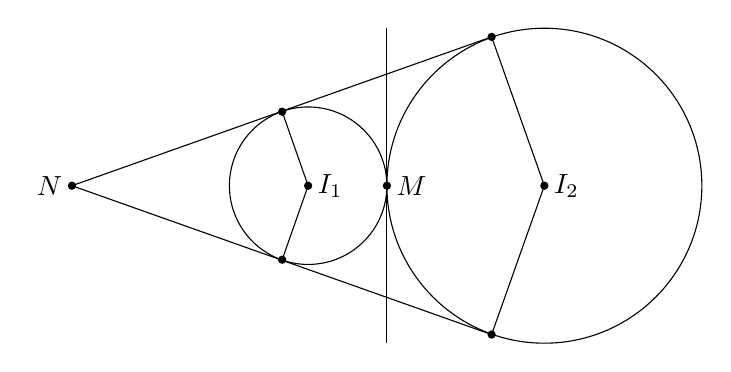
\begin{tikzpicture}
			\draw (1,0) circle (1cm);
			\draw (4,0) circle (2cm);
			\node at (1,0) [right] {$I_1$};
			\fill [fill = black] (1,0) circle (1.5pt);
			\node at (4,0) [right] {$I_2$};
			\fill [fill = black] (4,0) circle (1.5pt);
			\node at (-2,0) [left] {$N$};
			\fill [fill = black] (-2,0) circle (1.5pt);
			\draw (-2,0) -- (3.33, 1.89); \fill [fill = black] (3.33, 1.89) circle (1.5pt);
			\draw (-2,0) -- (3.33, -1.89); \fill [fill = black] (3.33, -1.89) circle (1.5pt);
			\draw (1,0) -- (0.67, 0.94); \fill [fill = black] (0.67, 0.94) circle (1.5pt);
			\draw (1,0) -- (0.67, -0.94); \fill [fill = black] (0.67, -0.94) circle (1.5pt);
			\draw (4,0) -- (3.33, 1.89);
			\draw (4,0) -- (3.33, -1.89);
			\draw (2,2) -- (2,-2);
			\node at (2,0) [right] {$M$}; \fill [fill = black] (2,0) circle (1.5pt);
	\end{tikzpicture}}
	\noindent Gọi $(P)$ là mặt phẳng tiếp xúc cả ba mặt cầu. $(P)$ đi qua $N$ và có véc-tơ pháp tuyến là $\overrightarrow n = (1;a;b)$.
	\begin{align*}
		\Rightarrow{} &\left( P \right) \colon x + 6 + a\left( {y - 2} \right) + b\left( {z - 4} \right) = 0 \\
		\Leftrightarrow{} &\left( P \right) \colon x + ay + bz - 2a - 4b + 6 = 0
	\end{align*}
	\noindent Tiếp tục, ta có
	\begin{align*}
		&\left\{ {\begin{array}{l}
				{d\left( {{I_1};(P)} \right) = 1} \\ 
				{d\left( {{I_2};(P)} \right) = 2} \\ 
				{d\left( {{I_3};(P)} \right) = 3} 
		\end{array}} \right. \\
		\Leftrightarrow{} &\left\{ \begin{array}{l}
			3 = \sqrt {1 + {a^2} + {b^2}} \\
			6 = 2\sqrt {1 + {a^2} + {b^2}} \\
			\left| {4b - 4} \right| = 3\sqrt {1 + {a^2} + {b^2}}  \hfill \\ 
		\end{array}  \right. \\
		\Leftrightarrow{} &\left[ \begin{gathered}
			b = \frac{{13}}{4} \hfill \\
			b =  - \frac{5}{4} \hfill \\ 
		\end{gathered}  \right.
	\end{align*}
	\noindent Với $b = \dfrac{13}{4} \Rightarrow a^2 = -\dfrac{41}{16}$ (loại).
	
	\noindent Với $b = -\dfrac{5}{4} \Rightarrow {a^2} = \dfrac{{103}}{{16}} \Rightarrow a =  \pm \dfrac{{\sqrt {103} }}{4}$.
	
	\noindent Vậy có $2$ mặt phẳng thoả mãn yêu cầu đề bài.
	}
\end{ex}
\Closesolutionfile{ans}
% \indapan{6}{ans/ans-2-B1}